\documentclass[12pt]{article}
	
\usepackage[margin=1in]{geometry}		% For setting margins
\usepackage{amsmath}				% For Math
\usepackage{fancyhdr}				% For fancy header/footer
\usepackage{graphicx}				% For including figure/image
\usepackage{cancel}					% To use the slash to cancel out stuff in work

%%%%%%%%%%%%%%%%%%%%%%
% Set up fancy header/footer
\pagestyle{fancy}
\fancyhead[LO,L]{Kate O'Neill - 21365768}
\fancyhead[CO,C]{CSU11031 - Electronics Assignment 3}
\fancyhead[RO,R]{\today}
\fancyfoot[LO,L]{}
\fancyfoot[CO,C]{\thepage}
\fancyfoot[RO,R]{}
\renewcommand{\headrulewidth}{0.4pt}
\renewcommand{\footrulewidth}{0.4pt}
%%%%%%%%%%%%%%%%%%%%%%
\begin{document}
\noindent Connect up the circuit below using Multisim (or CircuitLab if Multisim is not working) placing the voltmeters at the locations shown. Set the Process Transconductance (KP) to 0.02 (this is done by double clicking on the transistor giving you a menu on the right of the screen). You should use the NMOS 4T from the menu of components. Remember to connect the substrate to the Source.\\
\\
(i) Run the simulation. What do you observe? Please provide a superimposed plot of the node voltages using Grapher.\\
\begin{figure}[!h] 
	\begin{centering}
		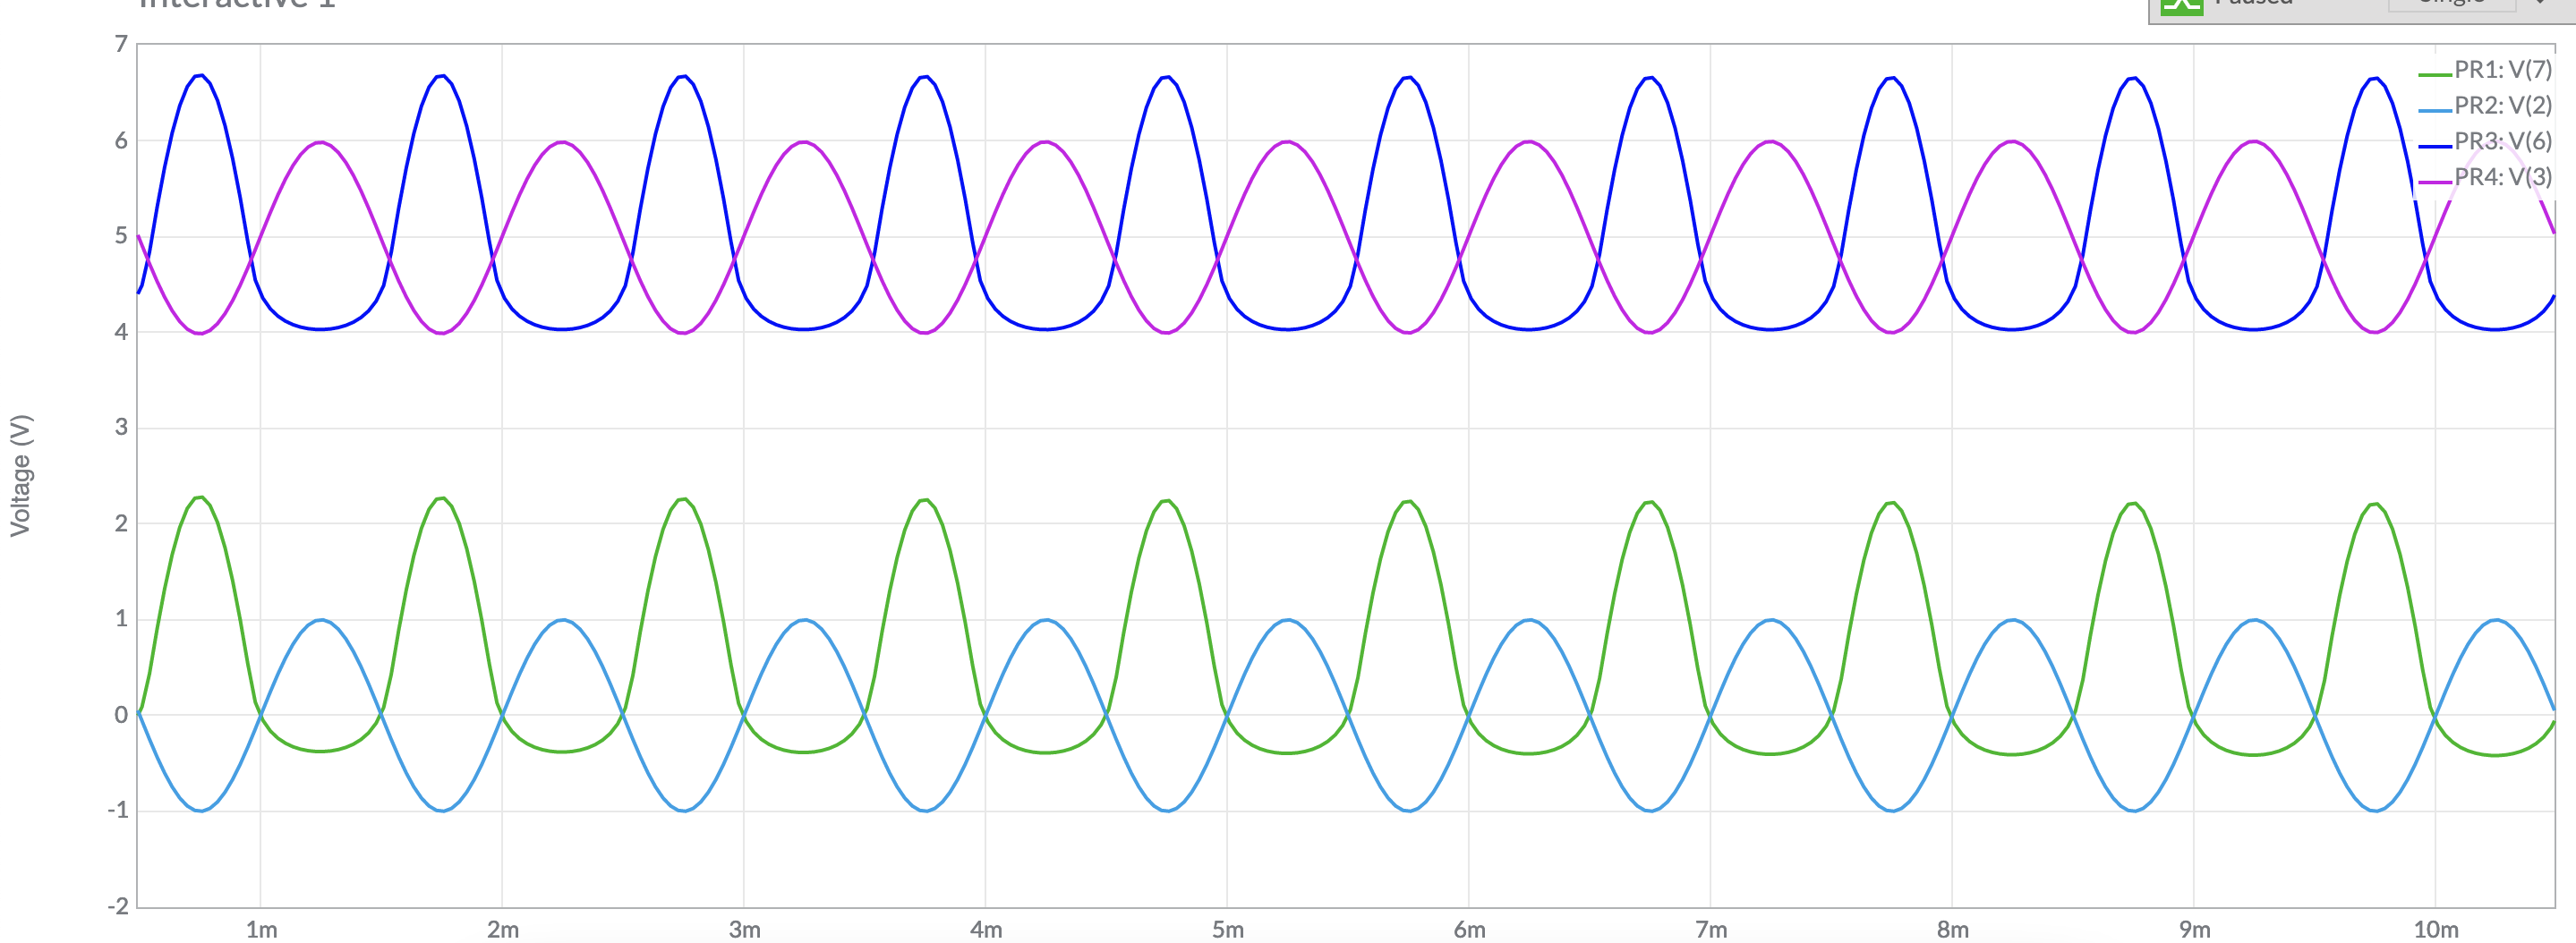
\includegraphics[keepaspectratio = true, width = 6in]{q1(i).png}
	\end{centering}
\end{figure}\\
Upon observation of the simulation, we can see that PR3 and PR4 have an almost perfect negative correlation, the same can be said for PR1 and PR2.\\
\\
(i) Calculate the voltage at the gate of the transistor. Does your answer tally with the result given in Grapher?\\
\\
Using \(V_G = (\frac{R4}{R3 + R4})V_{DD}\),\\
\[V_G = (\frac{100\times 10^3}{(200 \times 10^3) + (100 \times 10^3)})\times 15\]
\[V_G = 5V\]\\
\newpage
In order to verify this, we shall check the graph\\
\begin{figure}[!h] 
	\begin{centering}
		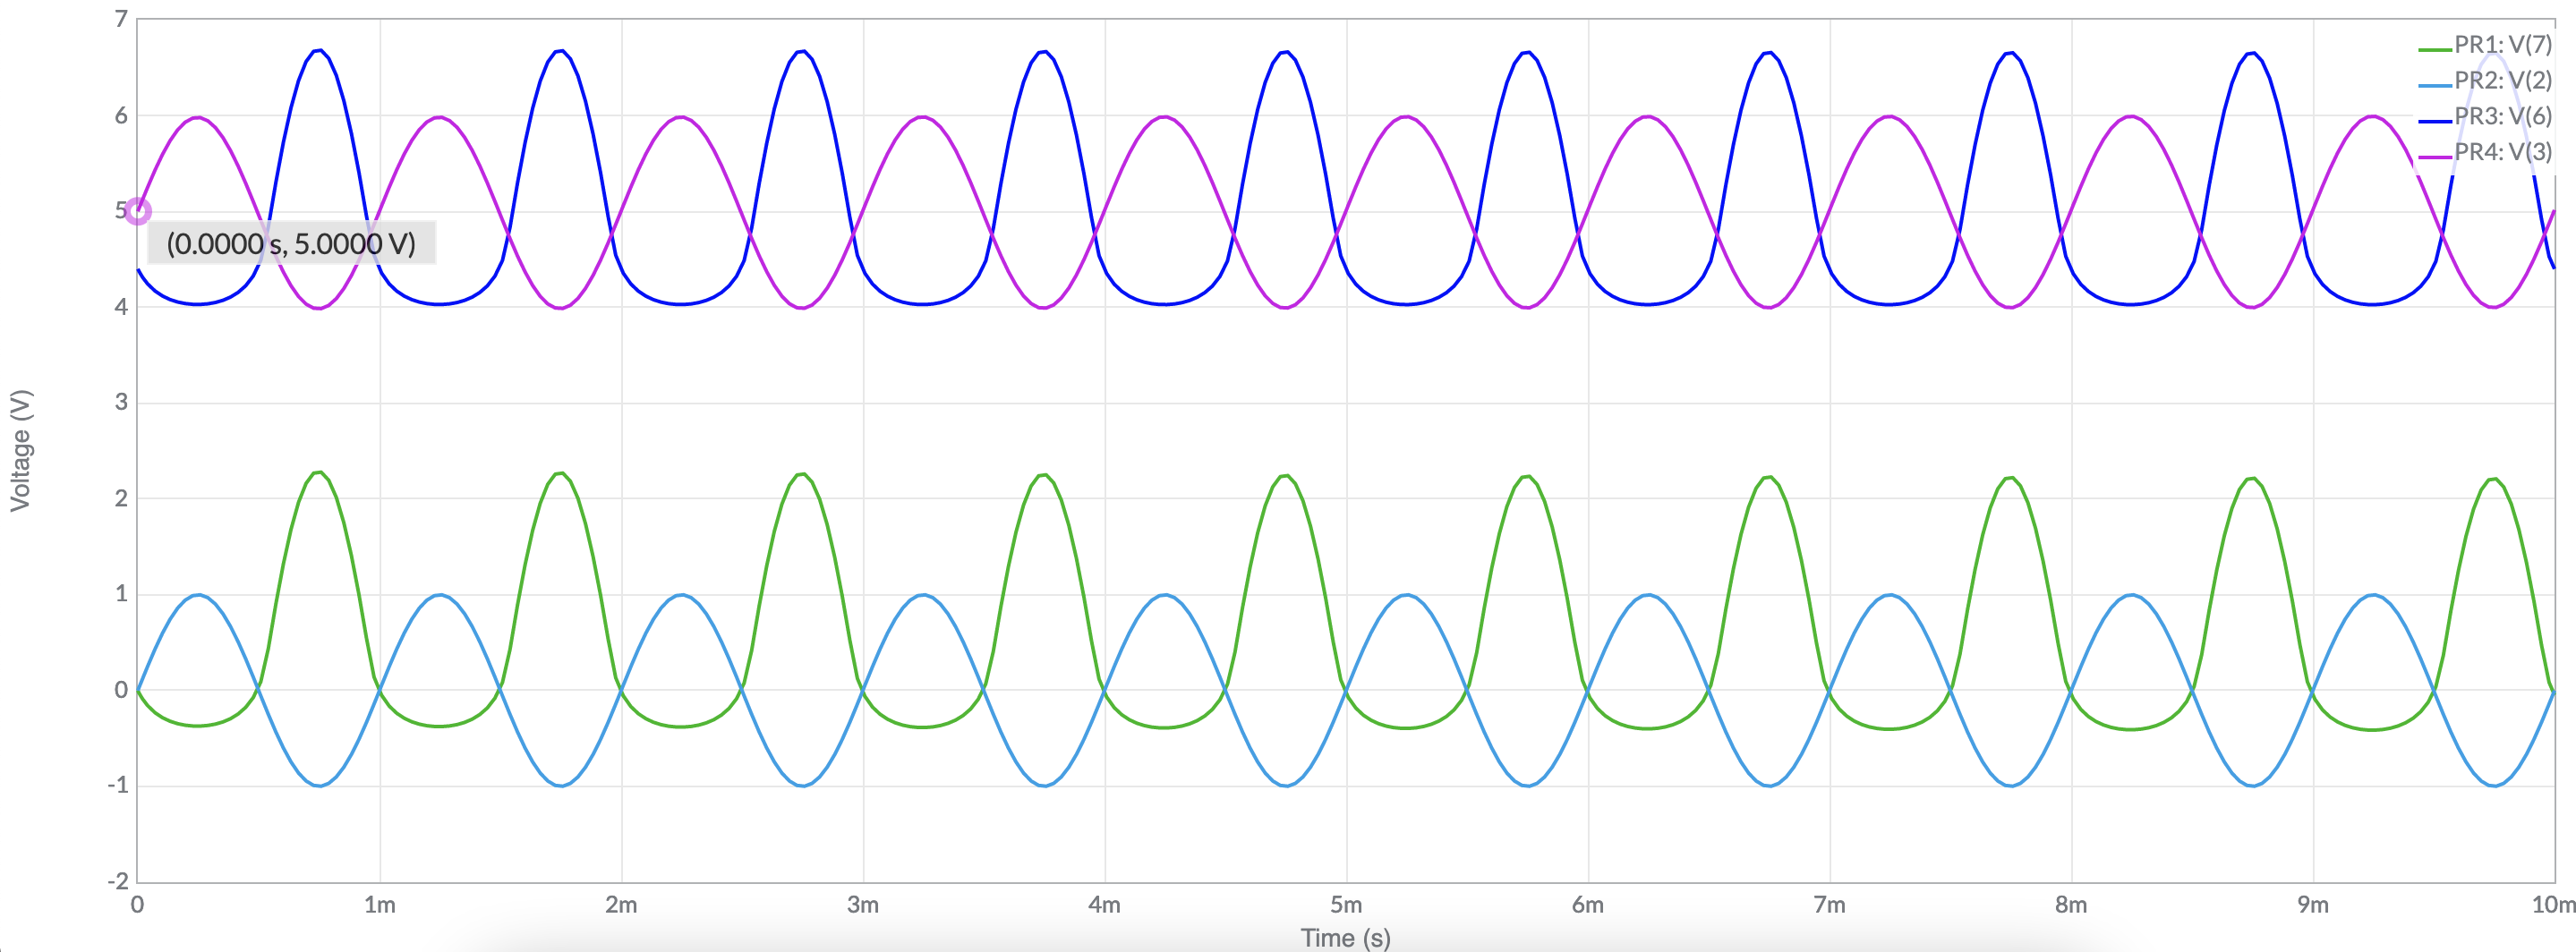
\includegraphics[keepaspectratio = true, width = 6in]{q1(ii).png}
	\end{centering}
\end{figure}\\
This coincides with our calculations, proving them to be correct.\\
\\
(iii) Observe the Drain voltage in Grapher. Explain why it has an a.c. and a d.c. component.\\
\\
The d.c. component prevents the transistor from switching off when the a.c components voltage drops.\\
\\
(iv) Explain the purpose of the capacitors at the input and the output.\\
\\
Capacitors are used to prevent current overflowing to the transistor, and are therefore crucial components in amplifier circuits such as this one. In essence, they isolate the d.c. signal, allowing the a.c. signal to pass.\\
\\
(v) You will observe that the output voltage is inverted with respect to the input voltage. Explain why this is so.\\
\\
As discussed previously, the graph shows an almost perfect inverse relationship between the input and output voltages. This is a feature of transistors. If a high voltage is inputted, then the transistor is turned on . If a low voltage is inputted, then the transistor is off.\\
\\
(vi) Estimate the gain of this amplifier?\\
\\
Using \(G = \frac{V_{in}}{V_{out}}\), where G is the gain of the amplifier, and the values of \(V_{in}\) and \(V_{out}\) are taken from the graph.\\
\[G = \frac{2.1545}{990.03 \times 10^{-3}}\]
\[G = 2.1762\]
\end{document}